\subsection{Solid Sphere}

A similar approach can then be employed for other solid shapes that can be broken down into shells or disks, such as a solid sphere with mass $M$ and radius $R$ shown in \cref{fig:rotating_solid_sphere}.

% !TEX root = ../math_ia.tex
\begin{figure}[H]
  \centering
  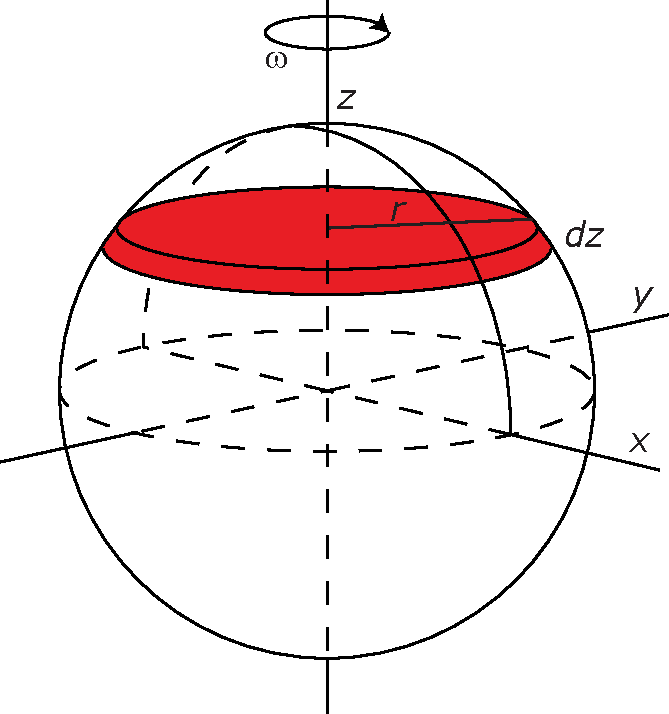
\includegraphics[width=0.25\linewidth]{fig/images/rotating_solid_sphere.pdf}
  \caption{A solid sphere centered at the origin rotating about the $Z$-axis with a constant angular velocity $\omega$. A small disk of radius $r$ has also been depicted for visualization purposes}
  \label{fig:rotating_solid_sphere}
\end{figure}

Again, assume the cylinder to have a constant density $\rho$, which can be written as:

\[\rho = \frac{M}{\frac{4}{3}\pi R^3}\]

Considering the thin disk with a radius $r$, we can write the infinitesmal moment of inertia for this disk by differentiating \cref{eq:final_moment_solid_cylinder}:

 \[dI = \frac{1}{2}r^2dm = \frac{1}{2}r^2\rho dV\]

 To calculate $dV$, a similar approach can be adopted by using the relation $V = A \times H$ and the fact that the height of this infinitesmal disk is simply $dz$:

 \[dV = \pi r^2 dz\]

 We can also relate the value of $z$, representing the height, with the value of $r$, representing the radius of the disk, using basic right-triangle geometry as the distance of all points on the sphere must be a distance of $R$ from the origin:

 \[r^2 + z^2 = R^2\]
 \[r^2 = R^2 - z^2\]

Plugging our values for $dV$ and $r^2$ back in and integrating from $-R$ to $R$ to travel from the bottom to the top of the sphere:

\[dI  = \frac{1}{2}r^2\rho dV = \frac{1}{2}r^2\rho \pi r^2 dz\]
\[I = \frac{1}{2}\rho \pi \int_{-R}^R r^4 dz\]
\[I = \frac{1}{2}\rho \pi \int_{-R}^R (R^2 - z^2)^2 dz\]
\[I =\frac{1}{2}\rho \pi \int_{-R}^R (R^4 + z^4 - 2R^2z^2) dz\]
\[I = \frac{1}{2}\rho \pi \left[\frac{z^5}{5} - \frac{2}{3}R^2z^3 + R^4z\right]_{-R}^{R}\]
\[I = \frac{8}{15}\rho \pi R^5\]

Substituting the initial value for $\rho$, the equation for the moment of inertia of solid cylinder can be derived as:

\begin{equation}
I_{\text{solid sphere}} = \frac{2}{5}MR^2
\label{eq:final_moment_solid_sphere}
\end{equation}